\chapter{Использование гауссовского сплаттинга для текстово-управляемого рендеринга}
\label{cha:text_to_3d}

В данном разделе рассматривается реализация текстово-управляемого рендеринга на основе гауссовского сплаттинга. Описываются ключевые компоненты системы, этапы интеграции CLIP-модели и процесс оптимизации параметров для генерации 3D-сцен по текстовым запросам.

\section{Архитектура реализации}

Гауссовский сплаттинг реализован как модульная система с чётким разделением ответственности между компонентами:

\begin{itemize}
    \item \textbf{Модель гауссиан.} Представляет сцену как набор 3D-гауссиан с параметрами:
    \begin{itemize}
        \item положение $\mathbf{p} \in \mathbb{R}^3$;
        \item ковариационная матрица $\Sigma \in \mathbb{R}^{3 \times 3}$;
        \item цвет $\mathbf{c} \in \mathbb{R}^3$;
        \item прозрачность $\alpha \in [0,1]$.
    \end{itemize}

    \item \textbf{Пайплайн рендеринга.} Выполняет проекцию 3D-гауссиан на 2D-изображение с учётом:
    \begin{itemize}
        \item матрицы камеры $W$ (world-to-camera transform);
        \item аффинного приближения при проекции на плоскость изображения;
        \item глубины и прозрачности для смешивания.
    \end{itemize}

    \item \textbf{CLIP-интеграция.} Связывает текстовое описание и изображение через общее эмбеддинг-пространство:
    \begin{itemize}
        \item эмбеддинги текста и изображения проецируются в общее пространство;
        \item используется косинусное расстояние в качестве функции потерь;
        \item применяется аугментация через случайные кропы.
    \end{itemize}

    \item \textbf{Оптимизатор.} Обновляет параметры гауссиан с помощью:
    \begin{itemize}
        \item градиентного спуска с использованием Adam;
        \item динамической адаптации плотности точек;
        \item периодического сброса прозрачности.
    \end{itemize}
\end{itemize}

\section{Выбор библиотек и инструментов}

Для реализации были выбраны следующие библиотеки:

\begin{itemize}
    \item \textbf{PyTorch} --- основа вычислений:
    \begin{lstlisting}[language=Python]
import torch
from torch.cuda.amp import autocast
    \end{lstlisting}

    \item \textbf{OpenCLIP} --- предобученные модели:
    \begin{lstlisting}[language=Python]
import open_clip
model, _, _ = open_clip.create_model_and_transforms('ViT-B-32', pretrained='laion2b_s34b_b79k')
    \end{lstlisting}

    \item \textbf{TorchVision} --- преобразования изображений:
    \begin{lstlisting}[language=Python]
from torchvision.transforms import Normalize
clippp = Normalize(mean=model.visual.image_mean, std=model.visual.image_std)
    \end{lstlisting}

    \item \textbf{NumPy} --- для численных операций:
    \begin{lstlisting}[language=Python]
import numpy as np
    \end{lstlisting}

    \item \textbf{Matplotlib + Celluloid} --- визуализация прогресса:
    \begin{lstlisting}[language=Python]
from celluloid import Camera
    \end{lstlisting}
\end{itemize}

\section{Создание и инициализация гауссиан}

\subsection{Генерация начальной сцены}

\begin{itemize}
    \item \textbf{Генерация координат.} Случайные точки $\mathbf{xyz} \in \mathbb{R}^{N \times 3}$ на единичной сфере:
    \[
        \mathbf{xyz}_{\text{norm}} = \frac{\mathbf{xyz}}{\|\mathbf{xyz}\|_2}, \quad N = 100,
    \]
    с масштабированием на коэффициент $1.3$.

    \item \textbf{Цвета через сферические гармоники (SH).} Используются SH-коэффициенты $\mathbf{shs} \in \mathbb{R}^{N \times 3}$:
    \[
        \text{SH2RGB}(\mathbf{x}) = \frac{1}{1 + e^{-k \cdot \mathbf{x}}}.
    \]

    \item \textbf{Создание объекта \texttt{BasicPointCloud}.}
    \begin{lstlisting}[language=Python]
pcd = BasicPointCloud(points=xyz, colors=SH2RGB(shs), normals=np.zeros((num_pts, 3)))
    \end{lstlisting}
\end{itemize}

\section{Интеграция CLIP}

\subsection{Обработка эмбеддингов}

\begin{itemize}
    \item Загрузка модели:
    \begin{lstlisting}[language=Python]
model = torch.jit.script(model).requires_grad_(False).cuda().half()
    \end{lstlisting}

    \item Нормализация изображений:
    \[
        \mu = [0.481, 0.457, 0.407], \quad \sigma = [0.268, 0.261, 0.275].
    \]

    \item Аугментация кропами:
    \[
        \mathbf{T} = \begin{bmatrix}
            s & 0 & t_x \\
            0 & s & t_y \\
            0 & 0 & 1
        \end{bmatrix}, \quad s \in [0.7, 0.9], \; t_x, t_y \in [0, 1 - s].
    \]

    \item Функция потерь:
    \[
        \mathcal{L}_{\text{CLIP}} = -\frac{1}{N} \sum_{i=1}^{N} \frac{\mathbf{v}_i^\top \mathbf{t}}{\|\mathbf{v}_i\| \cdot \|\mathbf{t}\|}.
    \]
    \begin{lstlisting}[language=Python]
sim = img_vec @ text_vec.T
clip_loss = -sim.mean()
    \end{lstlisting}
\end{itemize}

\section{Пайплайн рендеринга}

\begin{lstlisting}[style=pseudocode,caption={Rendering Pipeline for 3D Gaussians}]
procedure Render(w, h, M, S, C, A, V)
    (M_screen, S_screen) <- ScreenspaceGaussians(M, S, V)
    T <- TileGrid(w, h)
    (L, K) <- DuplicateWithKeys(M_screen, T)
    (L, K) <- SortByKeys(L, K)
    R <- ComputeTileRanges(T, K)
    I <- InitializeCanvas(w, h)
    for each tile t in T do
        for each pixel i in t do
            r <- GetTileRange(R, t)
            I[i] <- CompositeInOrder(i, L, r, K, M_screen, S_screen, C, A)
    return I
\end{lstlisting}


\section{Оптимизация и обучение}

\begin{itemize}
    \item Настройка гиперпараметров:
    \begin{lstlisting}[language=Python]
args.iterations = 2500
args.position_lr_init = 1e-2
args.position_lr_final = 1e-5
    \end{lstlisting}

    \item Обновление параметров:
    \begin{lstlisting}[language=Python]
gaussians.optimizer.step()
gaussians.optimizer.zero_grad(set_to_none=True)
    \end{lstlisting}

    \item Динамическая адаптация плотности:
    \begin{lstlisting}[language=Python]
gaussians.densify_and_prune(opt.densify_grad_threshold, 0.005, camera_extent, size_threshold)
if iteration % opt.opacity_reset_interval == 0:
    gaussians.reset_opacity()
    \end{lstlisting}

    \item Визуализация прогресса:
    \begin{lstlisting}[language=Python]
fig = plt.figure()
camera = PltCamera(fig)
camera.snap()
animation = camera.animate(blit=False, interval=50)
    \end{lstlisting}
\end{itemize}

\section{Пример использования}

\begin{itemize}
    \item Инициализация сцены: SH-цвета и случайные координаты.
    \item Рендеринг: с камеры, вращающейся вокруг объекта.
    \item Оптимизация: 2500 итераций градиентного спуска.
    \item Результат: визуализация в HTML5:
    \begin{lstlisting}[language=Python]
HTML(animation.to_html5_video())
    \end{lstlisting}
\end{itemize}
\section{Применение текстово-управляемого сплаттинга}

В данной части представлена практическая применение генерации 3D-сцены на основе текстового описания, используя гауссовский сплаттинг и интеграцию с моделью CLIP. В качестве примера рассматривается создание модели подсолнухов Ван Гога.

\subsection{Настройка и запуск обучения}

Текстовый запрос задаёт сцену: 

\begin{lstlisting}[language=Python]
prompt = "a 3d model of Van Gogh's Sunflowers, 3d asset, high quality, not noisy, beautiful, black background"
\end{lstlisting}

Параметры модели, пайплайна и оптимизации инициализируются через объекты \texttt{ModelParams}, \texttt{OptimizationParams} и \texttt{PipelineParams}. Задаются основные гиперпараметры:

\begin{lstlisting}[language=Python]
args.iterations = 2500
args.position_lr_init = 1e-2
args.position_lr_final = 1e-5
torch.manual_seed(2023)
\end{lstlisting}

Обучение запускается функцией \texttt{training()}, в которой происходит:

\begin{itemize}
    \item сопоставление изображения и текста через CLIP;
    \item оптимизация параметров гауссиан с помощью Adam;
    \item динамическая адаптация плотности облака точек;
    \item визуализация процесса обучения.
\end{itemize}

После завершения итераций результат сохраняется в HTML5-видео:

\begin{lstlisting}[language=Python]
HTML(animation.to_html5_video())
\end{lstlisting}

\subsection{Результат и анализ модели}

В результате реализованная система генерирует 3D-модель подсолнухов в виде облака гауссиан, соответствующего текстовому описанию. На рис.~\ref{fig:sunflowers_3d} представлен итог визуализации:

\begin{figure}[h!]
    \centering
    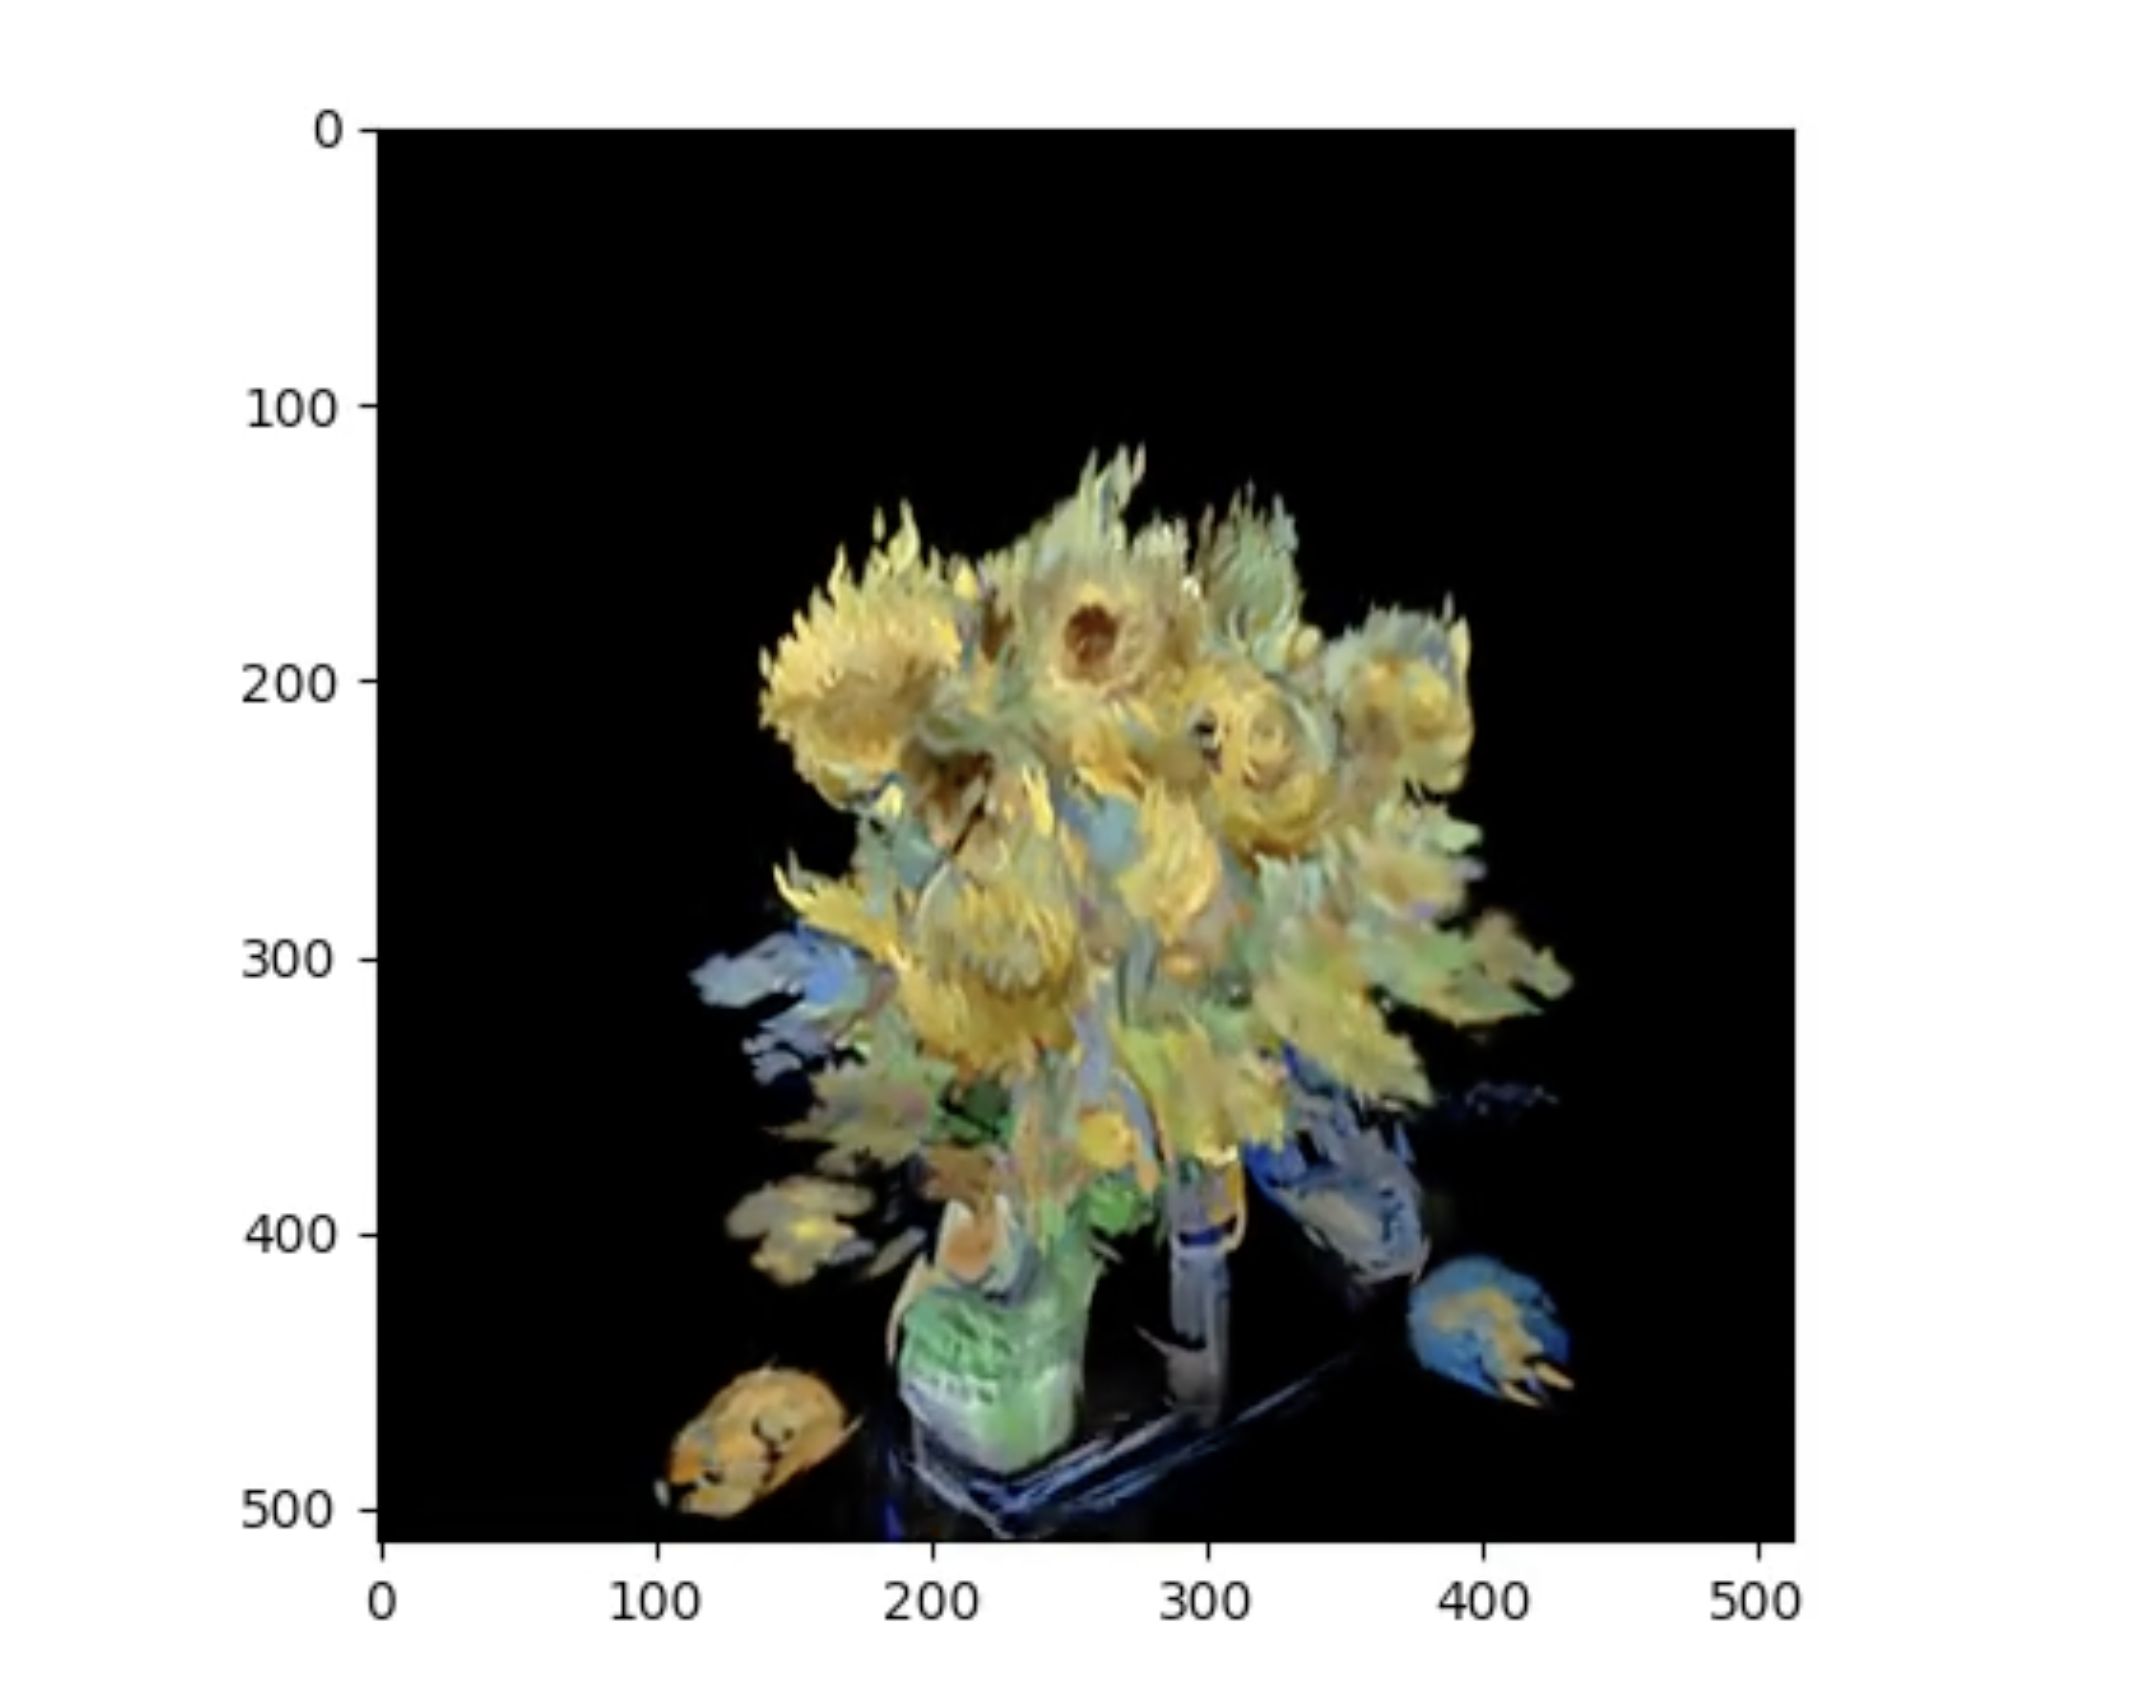
\includegraphics[width=0.6\textwidth]{sunflowers_3d_model.png}
    \caption{3D-модель подсолнухов Ван Гога, созданная с помощью текстово-управляемого гауссовского сплаттинга}
    \label{fig:sunflowers_3d}
\end{figure}

Полученная модель:

\begin{itemize}
    \item передаёт художественные особенности оригинальной сцены;
    \item поддерживает рендеринг с различных ракурсов;
    \item демонстрирует низкий уровень шума благодаря адаптивной плотности.
\end{itemize}

Таким образом, описанный подход подтверждает применимость гауссовского сплаттинга к задачам текстово-управляемой 3D-реконструкции, сочетая визуальную точность и эффективность дифференцируемого рендеринга.

